\begin{IEEEbiography}[{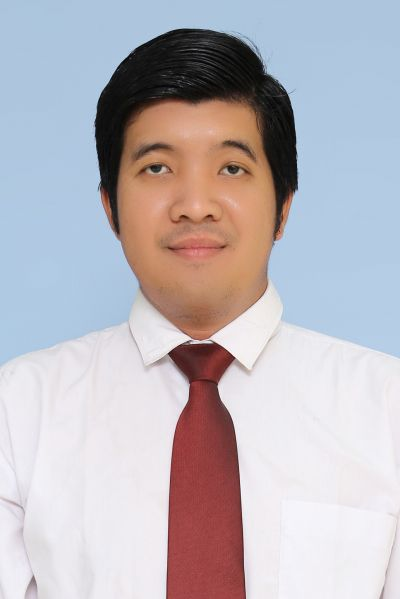
\includegraphics[width=1in,height=1.25in,clip,keepaspectratio]{images/author_ricky.jpg}}]{RICKY EKA PUTRA}
received the Bachelor's, Master's, and Doctoral degrees in Computer Science from Institut Teknologi Sepuluh Nopember (ITS) in 2008, 2011, and 2020, respectively, and obtained the Professional Engineer degree in 2024. Currently, he serves as a lecturer and researcher at the Department of Informatics, Faculty of Informatics, Universitas Negeri Surabaya. He is actively engaged in the implementation of the three pillars of higher education, encompassing informatics teaching, community empowerment programs, scientific publications in reputable journals, research dissemination at scientific seminars, and the acquisition of Intellectual Property Rights (IPR). His primary research focus is directed toward the development of applied artificial intelligence models that bridge advancements in intelligent computational methods with the resolution of real-world data-driven challenges. His research interests include Deep Learning, Computer Vision, Big Data Analytics, digital applications and user experience, clinical psychology, behavioral intention, healthcare informatics, statistical methods, as well as digital and early childhood education.
\end{IEEEbiography}

\begin{IEEEbiography}[{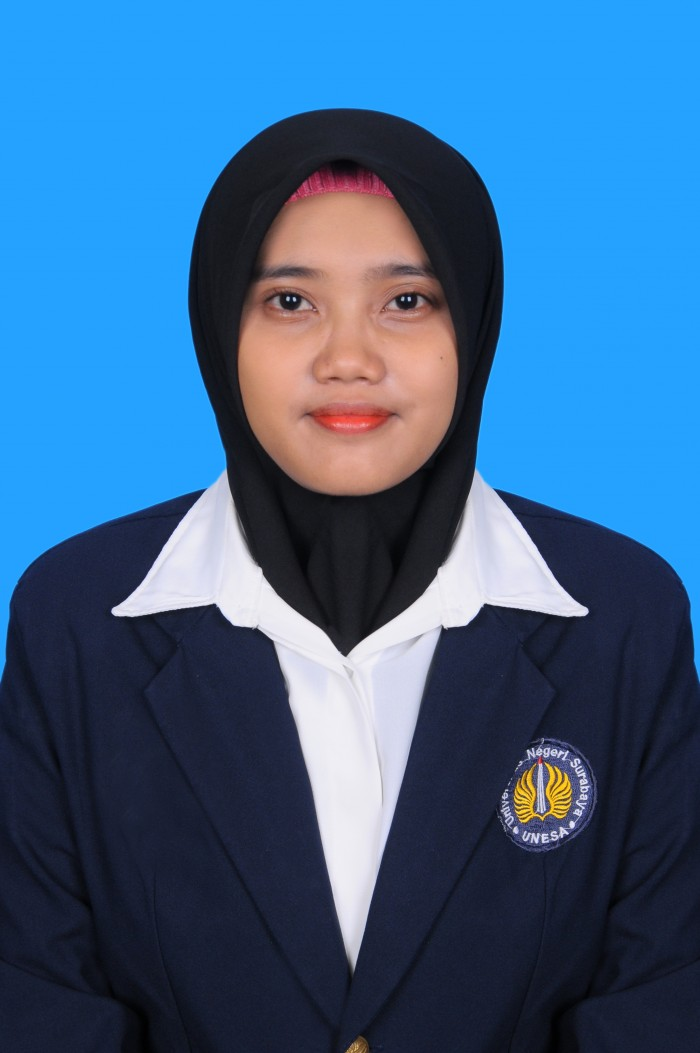
\includegraphics[width=1in,height=1.25in,clip,keepaspectratio]{images/author_rezky.jpg}}]{REZKY ARISANTI PUTRI}
received the Bachelor's degree in Informatics Engineering in 2019 with a specialization in Artificial Intelligence and completed her Master's degree in Informatics at Universitas Negeri Surabaya (UNESA). Currently, she actively serves as a researcher at the Department of Informatics, Faculty of Informatics, Universitas Negeri Surabaya. She is intensively involved in research on facial demographic attribute recognition based on transformer models and actively disseminates her scholarly contributions through publications in international conferences and reputable scientific journals. Her research focus and interests include Computer Vision, Deep Learning, Vision Transformers, Facial Attribute Recognition, Natural Language Processing, Machine Learning, and Algorithmic Fairness. Through consistent academic activities and research exploration, she continues to deepen her scientific competence and make tangible contributions to the advancement of intelligent computing technology.
\end{IEEEbiography}

\begin{IEEEbiography}[{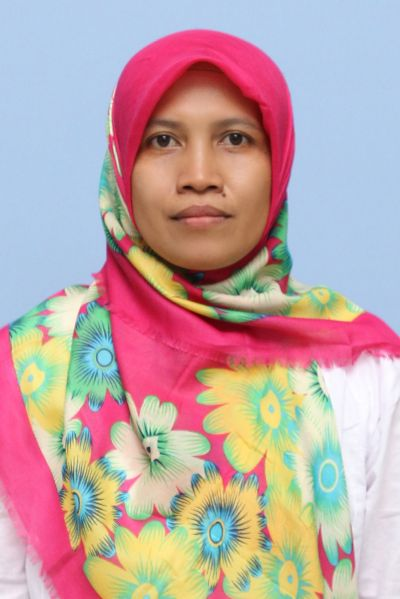
\includegraphics[width=1in,height=1.25in,clip,keepaspectratio]{images/author_yuni.jpg}}]{YUNI YAMASARI}
is a lecturer and researcher at the Department of Informatics, Faculty of Informatics, Universitas Negeri Surabaya (UNESA), with a solid academic foundation in both scholarly and practical domains. She received the Bachelor's, Master's, and Doctoral degrees from Institut Teknologi Sepuluh Nopember (ITS), with primary expertise in Software Engineering and Data Mining. Her activities across the three pillars of higher education are characterized by active involvement in community empowerment, publications of reputable scientific articles, and academic textbook authorship. She periodically disseminates her research findings across various national and international scientific forums and has acquired several Intellectual Property Rights (IPR). Her academic dedication is directed toward advancing software engineering, comprehensive data analysis, and applied informatics.
\end{IEEEbiography}

\begin{IEEEbiography}[{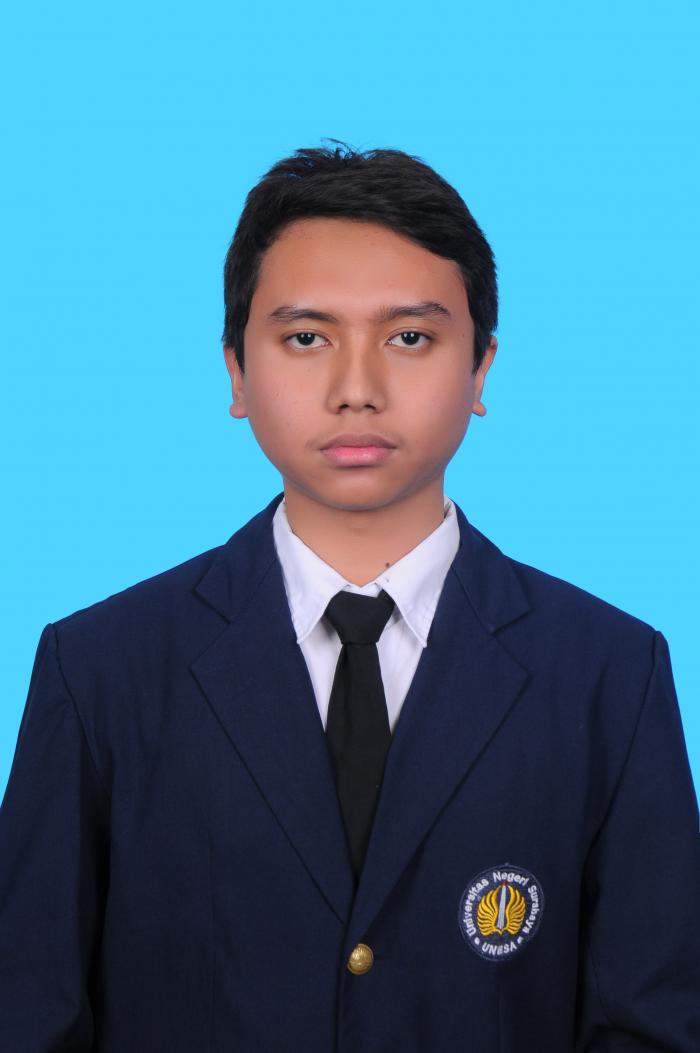
\includegraphics[width=1in,height=1.25in,clip,keepaspectratio]{images/author_rafy.jpg}}]{RAFY AULIA AKBAR}
received the Bachelor's degree in Informatics Engineering in 2019 and earned his Master's degree in Informatics from Universitas Negeri Surabaya with a concentration in Computer Science. During his studies, he achieved distinction by receiving the Best Solution Award at the regional competition ASEAN Vocational and Engineering Camp 2017 themed ``Toward School 4.0''. Currently, he actively dedicates himself as a researcher at the Department of Informatics, Faculty of Informatics, Universitas Negeri Surabaya. His research focus and interests center on the domains of Computer Vision, Medical Image Analysis, Multimodal Deep Learning, Natural Language Processing, and Vision Transformer architectures, particularly in the development of automated medical report generation systems.
\end{IEEEbiography}
